\documentclass{article}
\title{\bf \Huge The Sagemath Cloud\\ \textcolor{gray}{User Guide}}
\author{William Stein}

\usepackage{xcolor}
\usepackage{graphicx}
\usepackage{wrapfig}
\usepackage{hyperref}

\begin{document}
\maketitle
\tableofcontents
\newcommand{\smc}{Sagemath Cloud}

\section{Projects}

Once you create an \smc{} account, click on the Projects tab to see a
list of all projects that you are involved in.  This tab lists
any project that you either created or collaborate on, with the
most active projects listed at the top.



\begin{wrapfigure}{r}{.5\textwidth}
    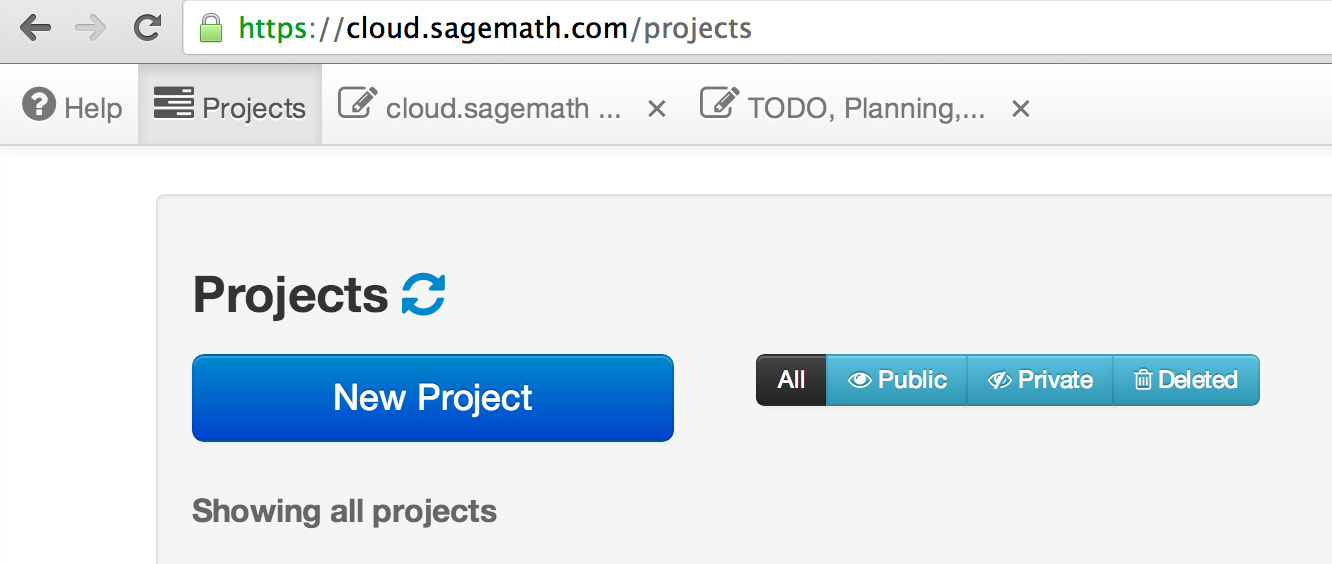
\includegraphics[width=.45\textwidth]{pics/project_tab}
\end{wrapfigure}
To create a new project, click the big ``New Project'' button and
fill in the title, description, and whether you want the project
to be public or private.  Don't worry too much about the tile, etc.,
since you can very easily change any of these settings at any time
later with no adverse effects.
Public projects can be viewed by anybody\footnote{As of Nov 3, 2013, public projects are not yet
visible to anybody, because this feature isn't completely implemented
yet.},
whereas private projects are only visible to you and
other collaborators on the project.


A project is the same thing as an account on some (very standard
Linux) computer.  Each project is completely self contained and isolated;
if you make changes to one project, this will not impact
other projects.

\begin{center}
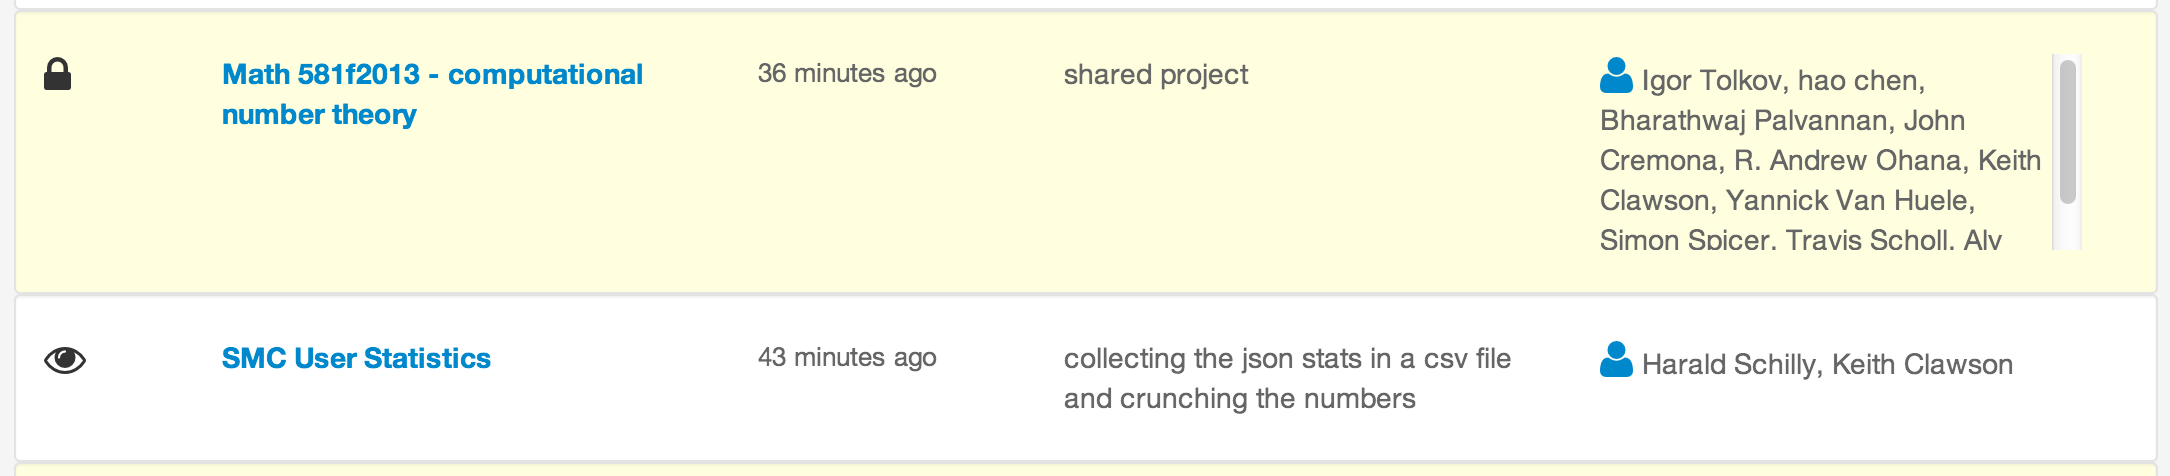
\includegraphics[width=.9\textwidth]{pics/projects}
\end{center}

There are five columns in the project listing.  The first is an
icon showing whether the project is public or private, the second
has the title, the third is the time since the project was last
modified, the fourth give the description of the project,
and the last column lists all collaborators on the project.
Click on the title of the project to open it.  If this is the first
time you've opened the project, or if you haven't opened it recently,
then it will usually take about 15 seconds to open the projects.
If you've opened it recently, it should open very quickly.
Alternatively, click on the list of collaborators on the right
(or the person icon, if the list is empty) to invite collaborators.


\section{Collaboration}

Collaborators have full access to the project; they can create and
edit any file, invite and remove
other collaborators, etc.  They {\em cannot} remove
the owner of the project from the project.

Often people will use the collaboration feature of a project in
order to ...
\begin{itemize}
\item {\em write a paper} using \LaTeX, but
with relevant documents, references, computations, also in
the project (see Section~\ref{sec:latex}).

\item as a scratch {\em common space for a course}.

\item securely {\em share a collection of IPython notebooks} (see
Section~\ref{sec:ipython}) or Sage
worksheets (see Section~\ref{sec:sagews})
with an explicit group of collaborators.
\item {\em develop code}: add a new feature to Sage (see Section~\ref{sec:sagedev}) or some
Python (or other) library (see Section~\ref{sec:pythondev}).  In this case, you may have several
subdirectories in the project, one for each person involved.
These directories might be separate git, svn or Mercurial
repositories.
\item {\em carry out a research project}: a student doing
research can collaborate with their adviser, who can open
the project and help them out when they run into issues.

\end{itemize}

\section{Navigating a Project}\label{sec:project}

\subsection{Files}
\subsection{Recent}

\subsection{New}
\subsection{Log}
\subsection{Project Settings}
\subsection{Search}

\subsection{Snapshots}

\section{Editing Files}\label{sec:files}

\subsection{Settings}

\section{\LaTeX{} documents}\label{sec:latex}

\section{Sage Worksheets}\label{sec:sagews}

\section{IPython Notebooks}\label{sec:ipython}

\section{Terminals}\label{sec:terminal}

\subsection{Settings}

\section{Python Development}\label{sec:sagedev}

\section{Sage Development}\label{sec:sagedev}

\section{Web Development}\label{sec:webdev}

\section{Using R: Statistical Computing}\label{sec:r}

\section{Using Octave}\label{sec:octave}

\section{Commercial Software}

\subsection{Mathematica}\label{sec:mathematica}

\subsection{Matlab}\label{sec:matlab}

\subsection{Maple}\label{sec:maple}

\subsection{Magma}\label{sec:magma}

\section{Other Mathematical Software}\label{sec:other}

\subsection{Axiom}

\subsection{GAP}

\subsection{Macaulay2}

\end{document}
%sagemathcloud={"zoom_width":150}